\documentclass{standalone}
\usepackage{pgfplots}
\pgfplotsset{compat=1.18}

\begin{document}
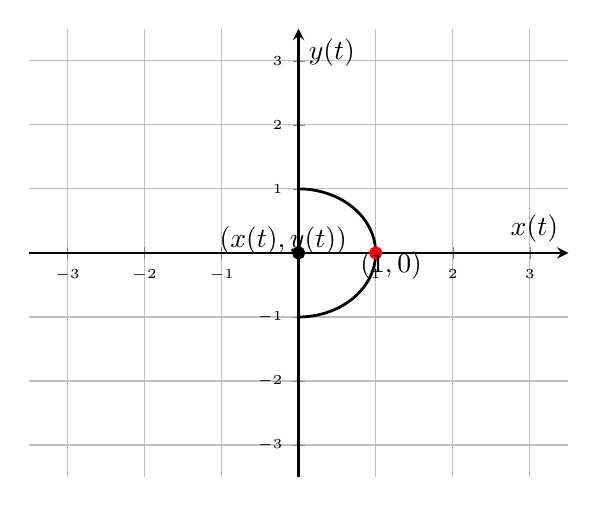
\begin{tikzpicture}
    \begin{axis}[
        axis lines = middle,
        xlabel = {$x(t)$},
        ylabel = {$y(t)$},
        xmin=-3.5, xmax=3.5,
        ymin=-3.5, ymax=3.5,
        grid=major,
        xtick={-3,-2,...,3},
        ytick={-3,-2,...,3},
        ticklabel style={font=\tiny},
        enlargelimits=false,
        clip=false,
        domain=-pi/2:pi/2,
        samples=200,
        no markers,
        smooth,
        thick,
        every axis plot/.append style={
            black,
            line width=1pt,
            mark options={fill=black}
        }
    ]
        \addplot [domain=-pi/2:pi/2] ({cos(deg(x))}, {sin(deg(x))});
        
        % Mark the point (1, 0)
        \filldraw[red] (1,0) circle (2pt);
        \node at (1.2, -0.2) {$(1, 0)$};
        
        % Label the point (x(t), y(t))
        \filldraw[black] (0,0) circle (2pt);
        \node at (-0.2, 0.2) {$(x(t), y(t))$};
    \end{axis}
\end{tikzpicture}
\end{document}